\subsection{use cases}
\label{sec:apusecase}
Here are the rest of the use cases based on our subsystems responsibility. 
\vspace{1em}

\subsubsection{Heartbeat System Robot Works}
\label{sec:heartbeat-works}

\begin{itemize}
    \item \textbf{Use Case Name:} Heartbeat System Robot Works
    \item \textbf{Actors:} Monitoring, Robot, Message Bus
    \item \textbf{Preconditions:} The robots, monitoring, and Message Bus system are up and running.
    \item \textbf{Steps:}
    \begin{itemize}[label=--]
        \item Monitoring system sends out a heartbeat to the Message Bus.
        \item Monitoring system waits about 1.5 seconds for a heartbeat return. 
        \item A Robot receives a heartbeat from the Message Bus and sends one in return. 
    \end{itemize}
    \item \textbf{Postconditions:} The monitoring system notes it has received a response, and a new heartbeat is sent in about 2 seconds.
\end{itemize}
\vspace{1em}

\subsubsection{Heartbeat System Robot Doesn't Work}
\label{sec:heartbeat-doesnt-work}

\begin{itemize}
\item \textbf{Use Case Name:} Heartbeat System Robot Doesn't Work
\item \textbf{Actors:} Monitoring, Robot, Message Bus
\item \textbf{Preconditions:} The robot is dead or non-responsive, monitoring, and Message Bus are running.
\item \textbf{Steps:}
\begin{itemize}[label=--]
\item Monitoring system sends out a heartbeat to the Message Bus.
\item Monitoring system waits about 1.5 seconds for a heartbeat return.
\item Robot does not send a return since it is non-responsive.
\end{itemize}
\item \textbf{Postconditions:} The monitoring system sends an error alert to the scheduler system.
\end{itemize}
\vspace{1em}

\subsubsection{Robot Receive Work Order}
\label{sec:robot-receive-work-order}

\begin{itemize}
\item \textbf{Use Case Name:} Robot Receive Work Order
\item \textbf{Actors:} Robot, Scheduler
\item \textbf{Preconditions:} Scheduler has a configured work order.
\item \textbf{Steps:}
\begin{itemize}[label=--]
\item The Scheduler sends the configured work order to the first Robot in the production line.
\item The Robot reads the robot function the scheduler has sent it and starts the work based on the function.
\end{itemize}
\item \textbf{Postconditions:} The robot finished the work and sends a response to the scheduler to start the next robot in the line.
\end{itemize}
\vspace{1em} 

\subsubsection{Configure the Order to Robot Function}
\label{sec:configure-order-to-robot-function}

\begin{itemize}
\item \textbf{Use Case Name:} Configure the Order to Robot Function
\item \textbf{Actors:} Configurate System, Scheduler
\item \textbf{Preconditions:} The scheduler has received an order, and the order parts are in inventory.
\item \textbf{Steps:}
\begin{itemize}[label=--]
\item The scheduler sends the order to the configurate system.
\item Configurate system configures the order details from simple strings to the appropriate robot functions for each robot.
\item Configurate sends the new configuration order back to the scheduler.
\end{itemize}
\item \textbf{Postconditions:} The scheduler inputs the work order into the schedule and waits for the robots to be able to work on the new order.
\end{itemize}
\vspace{1em} 

\subsubsection{Check Inventory System - Factory Does Have the Parts}
\label{sec:check-inventory-has-parts}

\begin{itemize}
\item \textbf{Use Case Name:} Check Inventory System - Factory Does Have the Parts
\item \textbf{Actors:} Scheduler System, Inventory System.
\item \textbf{Preconditions:} The Scheduler has received an order.
\item \textbf{Steps:}
\begin{itemize}[label=--]
\item Scheduler sends the order to the inventory system.
\item The inventory reads and converts the order strings into part numbers and amounts.
\item The part number and amount are then used to check the inventory of the factory.
\item The inventory system sends a message back that the parts are in, and green-lights for production.
\end{itemize}
\item \textbf{Postconditions:} The scheduling system sends the order to the configurator system since it has been greenlit for production.
\end{itemize}
\vspace{1em} 

\subsubsection{Check Inventory System - Factory Does Not Have the Parts}
\label{sec:check-inventory-no-parts}

\begin{itemize}
\item \textbf{Use Case Name:} Check Inventory System - Factory Does Not Have the Parts
\item \textbf{Actors:} Scheduler System, Inventory System.
\item \textbf{Preconditions:} The Scheduler has received an order.
\item \textbf{Steps:}
\begin{itemize}[label=--]
\item Scheduler sends the order to the inventory system.
\item The inventory reads and converts the order strings into part numbers and amounts.
\item The part number and amount are then used to check the inventory of the factory.
\item The inventory system sends a message back that the parts are not in the inventory and to hold off on production.
\end{itemize}
\item \textbf{Postconditions:} The scheduling system sends an update message to the order database that the order is not ready for production since the parts are not in-house.
\end{itemize}
\vspace{1em} 

\subsubsection{New Functionality Is Added to the System}
\label{sec:new-functionality-added}

\begin{itemize}
\item \textbf{Use Case Name:} New Functionality Is Added to the System
\item \textbf{Actors:} Developer, System, and Script Deployment Commands
\item \textbf{Preconditions:} The script deployment commands are up-to-date, the build server is up and running.
\item \textbf{Steps:}
\begin{itemize}[label=--]
\item The developer, after having developed a feature in their own branch and a test the feature, pushes to main.
\item The script deployment commands build, tests.
\item If the tests are good, the code is then deployed to the build server.
\end{itemize}
\item \textbf{Postconditions:} The new feature is now up and running in the system.
\end{itemize}

\subsubsection{Admin stop/change production}
\label{sec:admin-stop-change}

\begin{itemize}
\item \textbf{Use Case Name:} Admin stop/change production
\item \textbf{Actors:} Admin, scheduler, inventory system 
\item \textbf{Preconditions:} There are  orders in the schedule or in the order database, admin is loged in to the admin interface
\item \textbf{Steps:}
\begin{itemize}[label=--]
\item The admin goes and change or removes and order in the schedule, 
\item The scheduler Changed the schedule to fit the change
\item If The change is with the parts the scheduler calls the inventory system if new parts are needed
\end{itemize}
\item \textbf{Postconditions:} The production system goes with the changed schedule 
\end{itemize}

\newpage
\subsection{QAS}
\label{sec:QAS}

Here are all the Quality attribute scenarios in a bigger format
\vspace{1em}
\subsubsection{Availability QAS}
\label{sec:avaqas}
\textcolor{white}{somting}
\begin{figure}[H]
    \centering
    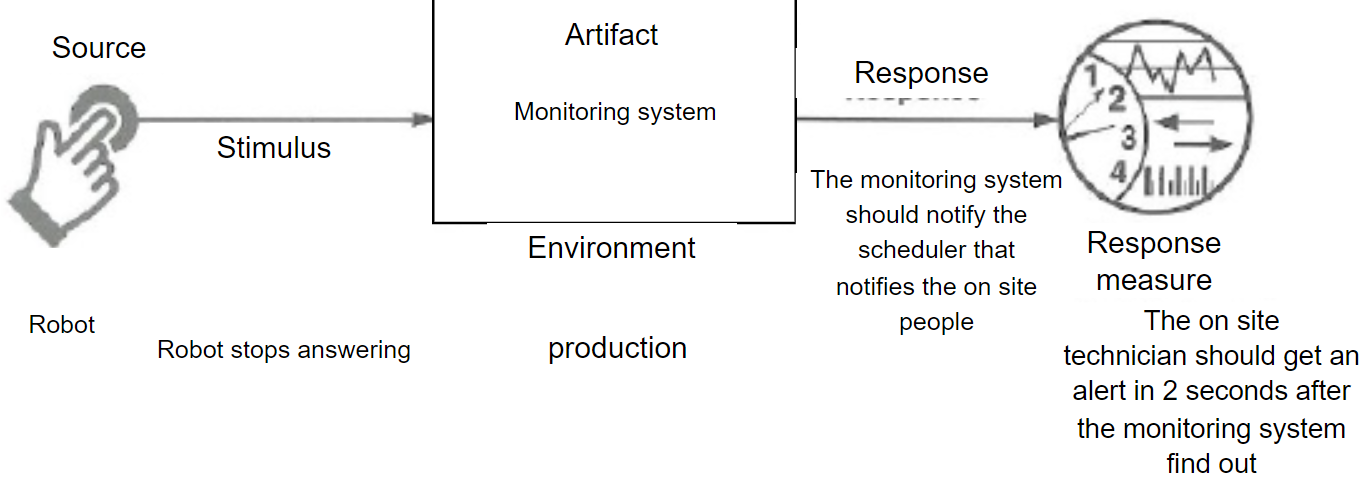
\includegraphics[width=0.8\linewidth]{Images/availability.png}
    \label{fig:availability}
\end{figure}

\subsubsection{Deployability QAS}
\label{sec:deployqas}
\textcolor{white}{somting}
\begin{figure}[H]
    \centering
    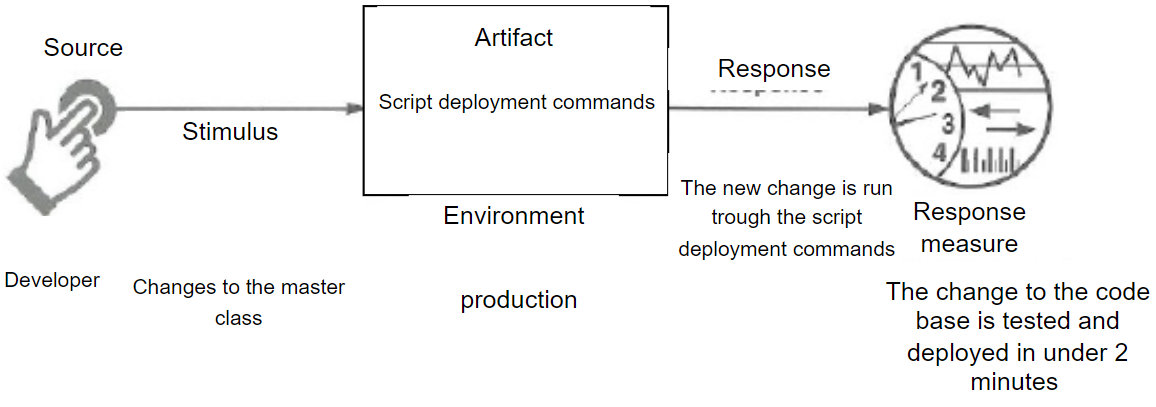
\includegraphics[width=0.8\linewidth]{Images/Deployability.png}
    \label{fig:deployability}
\end{figure}

\subsubsection{Performance QAS}
\label{sec:performanceqas}
\textcolor{white}{somting}
\begin{figure}[H]
    \centering
    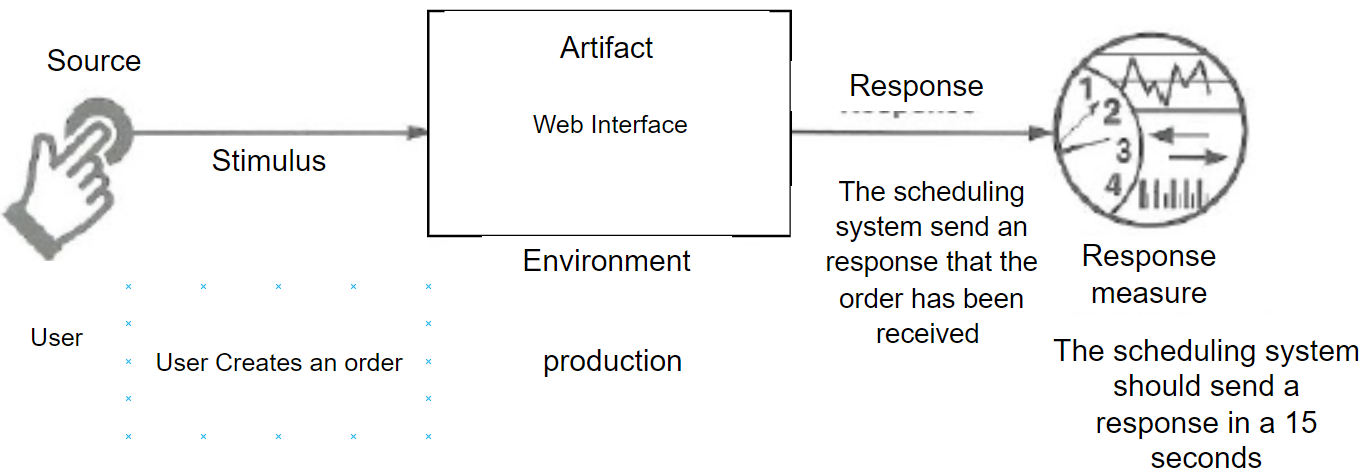
\includegraphics[width=0.8\linewidth]{Images/Performance.png}
    \label{fig:performance}
\end{figure}

\subsubsection{scalability QAS}
\label{sec:scalabilityqas}
\textcolor{white}{somting}
\begin{figure}[H]
    \centering
    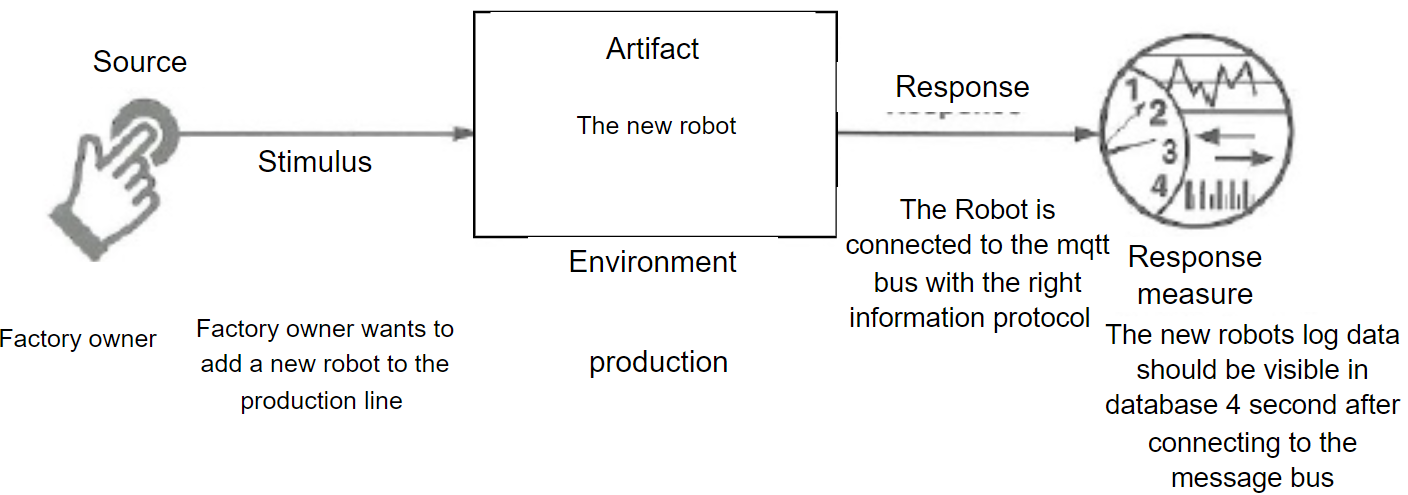
\includegraphics[width=0.8\linewidth]{Images/scalability.png}
    \label{fig:scalability}
\end{figure}

\subsection{Systemdiagram}
\label{sec:systemdiagram}
\begin{figure}[H]
    \centering
    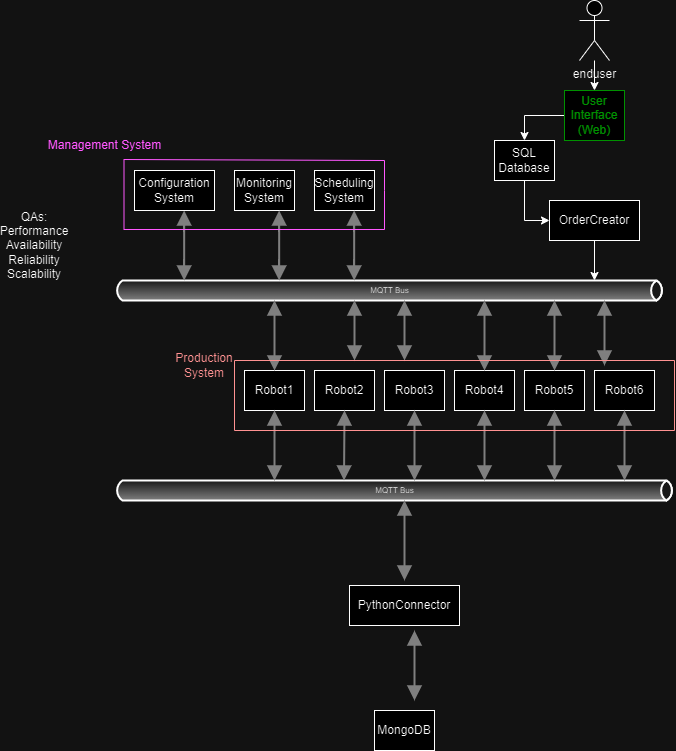
\includegraphics[width=0.8\linewidth]{Images/Systemdiagram.drawio.png}
    \label{fig:systemdiagram}
\end{figure}

\newpage

\subsection{Test results}
\label{sec:testresults}
\vspace{1em}
\begin{center}
    \begin{table}[H]
\begin{tabular}{|c|c|}
\hline
\multicolumn{1}{|l|}{Test number} & \multicolumn{1}{l|}{Test Result} \\ \hline
1 & 1.94289708137512 \\ \hline
2 & 2.00260353088378 \\ \hline
3 & 3.1728389263153 \\ \hline
4 & 2.77249479293823 \\ \hline
5 & 3.42909026145935 \\ \hline
6 & 3.08505964279174 \\ \hline
7 & 3.47967600822448 \\ \hline
8 & 3.36703920364379 \\ \hline
9 & 1.73941993713378 \\ \hline
10 & 3.13166284561157 \\ \hline
11 & 2.15875387191772 \\ \hline
12 & 1.52704811096191 \\ \hline
13 & 1.86307263374328 \\ \hline
14 & 2.63568592071533 \\ \hline
15 & 1.53997063636779 \\ \hline
16 & 1.6852867603302 \\ \hline
17 & 2.85078358650207 \\ \hline
18 & 2.18345427513122 \\ \hline
19 & 1.98611140251159 \\ \hline
\multicolumn{1}{|l|}{\textbf{Average of the test}} & \textbf{2.450155233} \\ \hline
\end{tabular}
\end{table}
\end{center}


\subsection{Github workflow}
\label{sec:github_workflow}
\begin{figure}[H]
    \centering
    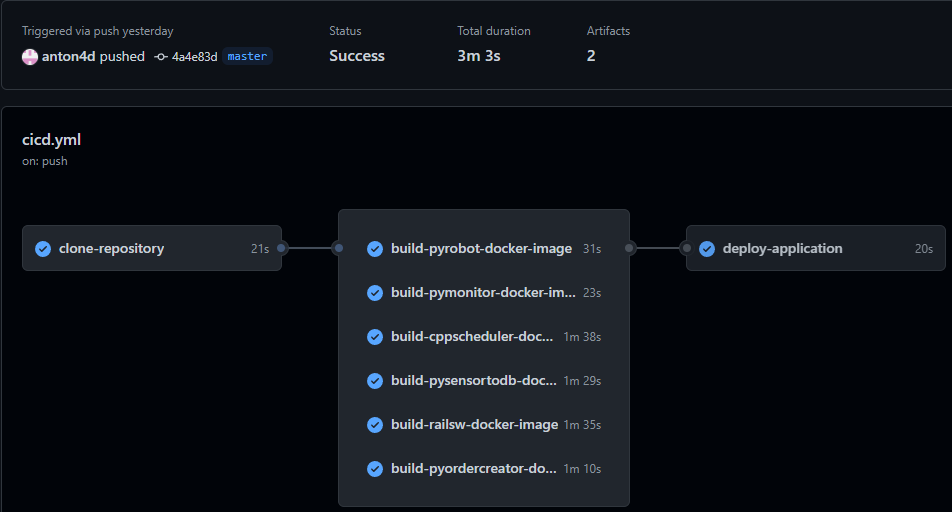
\includegraphics[width=0.8\linewidth]{Images/Github-Workflow.png}
    \label{fig:systemdiagram}
\end{figure}


